% !TEX TS-program = pdflatex
% !TEX encoding = UTF-8 Unicode

% This is a simple template for a LaTeX document using the "article" class.
% See "book", "report", "letter" for other types of document.

\documentclass[11pt]{article} % use larger type; default would be 10pt

\usepackage[utf8]{inputenc} % set input encoding (not needed with XeLaTeX)

%%% Examples of Article customizations
% These packages are optional, depending whether you want the features they provide.
% See the LaTeX Companion or other references for full information.

%%% PAGE DIMENSIONS
\usepackage{geometry} % to change the page dimensions
\geometry{a4paper} % or letterpaper (US) or a5paper or....
% \geometry{margins}{2cm} % for example, change the margins to 2 inches all round
% \geometry{landscape} % set up the page for landscape
%   read geometry.pdf for detailed page layout information

\usepackage{graphicx} % support the \includegraphics command and options
\usepackage{hyperref}

\usepackage[parfill]{parskip} % Activate to begin paragraphs with an empty line rather than an indent

%%% PACKAGES
\usepackage{booktabs} % for much better looking tables
\usepackage{array} % for better arrays (eg matrices) in maths
\usepackage{paralist} % very flexible & customisable lists (eg. enumerate/itemize, etc.)
\usepackage{verbatim} % adds environment for commenting out blocks of text & for better verbatim
\usepackage{subfig} % make it possible to include more than one captioned figure/table in a single float
% These packages are all incorporated in the memoir class to one degree or another...

% Colored tables
\usepackage{color}
\usepackage{colortbl}

% Configure fancyvrb for our listings
\usepackage{fancyvrb}
\fvset{frame=leftline, framesep=5mm, tabsize=8, numbers=left}

%%% HEADERS & FOOTERS
\usepackage{fancyhdr} % This should be set AFTER setting up the page geometry
\pagestyle{fancy} % options: empty , plain , fancy
\renewcommand{\headrulewidth}{0pt} % customise the layout...
\lhead{}\chead{}\rhead{}
\lfoot{}\cfoot{\thepage}\rfoot{}

%%% SECTION TITLE APPEARANCE
\usepackage{sectsty}
\allsectionsfont{\sffamily\mdseries\upshape} % (See the fntguide.pdf for font help)
% (This matches ConTeXt defaults)

%%% ToC (table of contents) APPEARANCE
\usepackage[nottoc,notlof,notlot]{tocbibind} % Put the bibliography in the ToC
\usepackage[titles,subfigure]{tocloft} % Alter the style of the Table of Contents
\renewcommand{\cftsecfont}{\rmfamily\mdseries\upshape}
\renewcommand{\cftsecpagefont}{\rmfamily\mdseries\upshape} % No bold!

%%% END Article customizations

%%% The "real" document content comes below...

\title{Mumble protocol 1.2.X reference (WIP)}
\author{Stefan Hacker}
%\date{} % Activate to display a given date or no date (if empty),
         % otherwise the current date is printed 

\newenvironment{mumbleMessage}[1]
{%
\begin{center}
	\begin{tabular}{|p{0.2\textwidth}|p{0.15\textwidth}|}
	%\begin{tabular}{|l|l|}
	\hline
	\multicolumn{2}{|>{\columncolor[rgb]{0.5,0.75,1}}l|}{\textbf{#1}} \\
	\hline
}
{%
	\\ \hline
	\end{tabular}
\end{center}
}

% \newcommand{\mumbleMessage}[2]{ #1 & #2 \\ }

\begin{document}
\maketitle

\newpage
\section*{DISCLAIMER}

THIS DOCUMENTATION IS PROVIDED BY THE MUMBLE PROJECT "AS IS" AND ANY EXPRESS OR IMPLIED WARRANTIES, INCLUDING, BUT NOT LIMITED TO, THE IMPLIED WARRANTIES OF MERCHANTABILITY AND FITNESS FOR A PARTICULAR PURPOSE ARE DISCLAIMED. IN NO EVENT SHALL THE MUMBLE PROJECT BE LIABLE FOR ANY DIRECT, INDIRECT, INCIDENTAL, SPECIAL, EXEMPLARY, OR CONSEQUENTIAL DAMAGES (INCLUDING, BUT NOT LIMITED TO, PROCUREMENT OF SUBSTITUTE GOODS OR SERVICES; LOSS OF USE, DATA, OR PROFITS; OR BUSINESS INTERRUPTION) HOWEVER CAUSED AND ON ANY THEORY OF LIABILITY, WHETHER IN CONTRACT, STRICT LIABILITY, OR TORT (INCLUDING NEGLIGENCE OR OTHERWISE) ARISING IN ANY WAY OUT OF THE USE OF THIS DOCUMENTATION, EVEN IF ADVISED OF THE POSSIBILITY OF SUCH DAMAGE. 

\tableofcontents
\newpage

\section{Introduction}
This document is meant to be a reference for the Mumble VoIP 1.2.X server-client communication protocol. It reflects the state of the protocol implemented in the Mumble 1.2.2 client and might be outdated by the time you are reading this. Be sure to check for newer revisions of this document on our website \url{http://www.mumble.info} . At the moment this document is work in progress.

\section{Overview}

\begin{figure}[ht]
	\centering
	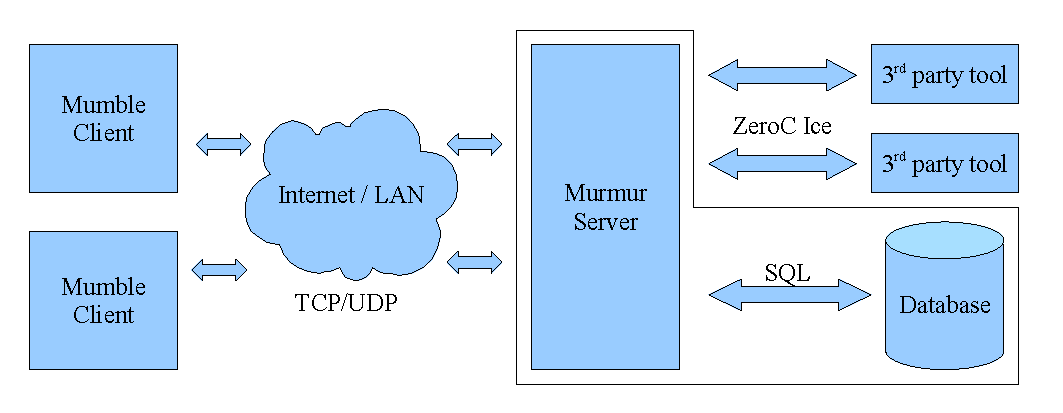
\includegraphics[width=\linewidth]{resources/mumble_system_overview}
	\caption{Mumble system overview}
	\label{fig:mumble_system_overview}
\end{figure}

Mumble is based on a standard server-client communication model. It utilizes two channels of communication, the first one is a TCP connection which is used to reliably transfer control data between the client and the server. The second one is a UDP connection which is used for unreliable, low latency transfer of voice data.

\begin{figure}[ht]
	\centering
	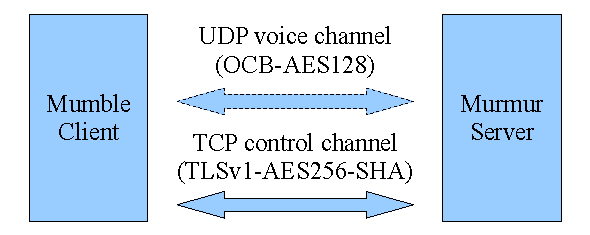
\includegraphics[width=0.5\linewidth]{resources/mumble_crypt_types}
	\caption{Mumble crypto types}
	\label{fig:mumble_crypt_types}
\end{figure}

Both are protected by strong cryptography, this encryption is mandatory and cannot be disabled. The TCP control channel uses TLSv1 AES256-SHA\footnote{\url{http://en.wikipedia.org/wiki/Transport_Layer_Security }} while the voice channel is encrypted with OCB-AES128\footnote{\url{http://www.cs.ucdavis.edu/~rogaway/ocb/ocb-back.htm}}.

While the TCP connection is mandatory the UDP connection can be compensated by tunnelling the UDP packets through the TCP connection as described in the protocol description later.

\section{Protocol stack (TCP)}

\begin{figure}[ht]
	\centering
	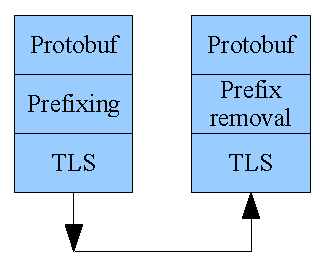
\includegraphics[width=0.3\linewidth]{resources/mumble_protocol_stack}
	\caption{Mumble protocol stack}
	\label{fig:mumble_protocol_stack}
\end{figure}

Mumble has a shallow and easy to understand stack. Basically it uses Googles Protocol Buffers\footnote{\url{http://code.google.com/p/protobuf/}} with simple prefixing to distinguish the different kinds of packets sent through an TLSv1 encrypted connection. This makes the protocol very easily expandable.

\begin{figure}[ht]
	\centering
	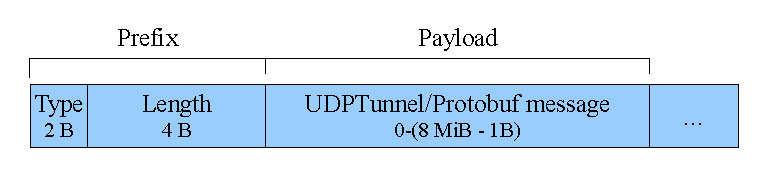
\includegraphics[width=0.8\linewidth]{resources/mumble_packet}
	\caption{Mumble packet}
	\label{fig:mumble_packet}
\end{figure}

The prefix consists out of the two bytes defining the type of the packet in the payload and 4 bytes stating the length of the payload in bytes followed by the payload itself. The following packet types are available in the current protocol and all but UDPTunnel are simple protobuf messages. If not mentioned otherwise all fields are little-endian encoded.

%FIGURE GOES HERE

For raw representation of each packet type see the attached Mumble.proto file.

\section{Establishing a connection}
The following section is going to describe the communication between the server and the client during connection establishing, note that the first part of this section only contains the procedures for the TCP connection. After this the client will be visible to the other clients on the server and able to send other types of messages.

\begin{figure}[ht]
	\centering
	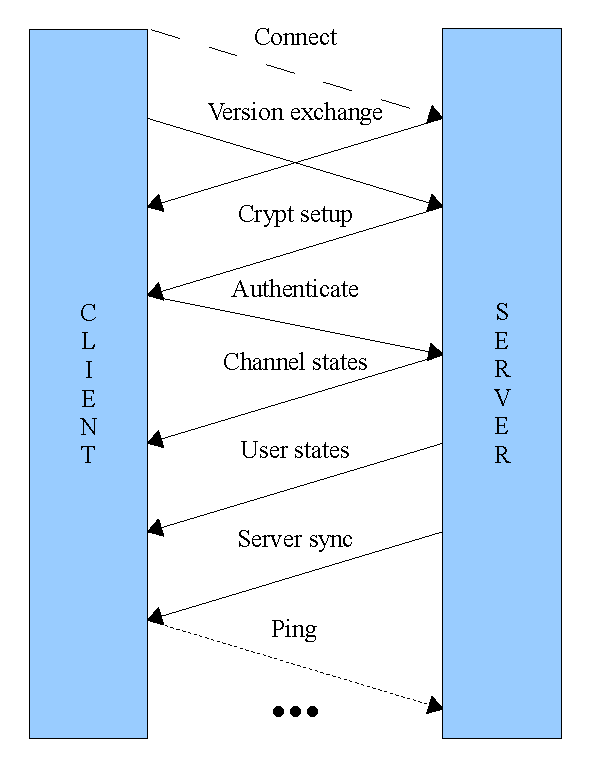
\includegraphics[width=0.7\linewidth]{resources/mumble_connection_setup}
	\caption{Mumble connection setup}
	\label{fig:mumble_connection_setup}
\end{figure}

\subsection{Connect}
As a basis for the synchronization procedure you first have to establish the TCP connection to the server and do a common TLSv1 handshake. To be able to use the complete feature set of the Mumble protocol it is recommended that your client provides a strong certificate to the server. This however is not mandatory, you can connect to the server without providing a certificate, we do recommend to check the servers certificate though.

\subsection{Version exchange}
Once the TLS handshake is completed the server will send a Version packet to the client containing following information:

\begin{mumbleMessage}{Version}
	version		& uint32 \\
	release		& string \\
	os			& string \\
	os\_version	& string
\end{mumbleMessage}


The client is supposed to send a Version packet with his information before any other messages. The version field of the packet contains the (major, minor, patch) tuple (e.g. 1.2.0) encoded like described in the following figure.

\begin{center}\begin{tabular}{|@{\hspace{0.5cm}}c@{\hspace{0.5cm}}|c|c|}
\hline
Major	& Minor	& Patch \\
2B		& 1B	& 1B \\
\hline
\end{tabular}\end{center}

The release, os and os\_version fields are common strings containing additional information about the client. This information is not interpreted in any way at the moment.

\subsection{Crypt setup}
Once the Version packets are exchanged the server will send a CryptSetup packet to the client. It contains the necessary cryptographic information to establish the OCB-AES128 encrypted UDP Voice channel. This will be described later in the section.

\begin{mumbleMessage}{CryptSetup}
	Key			& ByteString \\
	ServerNonce	& ByteString \\
	ClientNonce	& ByteString
\end{mumbleMessage}

\subsection{Authenticate}
Before the client can be synchronized with the server state it has to authenticate itself to the server. This is done by sending an Authenticate packet.

\begin{mumbleMessage}{Authenticate}
	username	& string \\
	password	& string \\
	tokens		& repeated string
\end{mumbleMessage}

The username and password are encoded as simple strings. Be aware that the server can impose restrictions on the username, also once the client registered a certificate with the server this field is only displayed in brackets behind the name the client posessed when he registered, for more information see the server documentation. The password must only be provided if the server is passworded, the client provided no certificate but wants to authenticate to an account which has a password set, or to access the SuperUser account. The third field called tokens contains a list of zero or more strings called tokens which are basically password which can give you access to a certain ACL group without actually being a registered member in them, again see the server documentation for more information.

\subsection{Channel states}

After the client is successfully authenticated the server starts synchronizing the state by transmitting a ChannelState message for every channel on this server. Note that these do not yet contain channel links. These are transmitted as updated directly after every channel has been transmitted. It contains the following information:

%FIGURE GOES HERE
For more information pease refer to \nameref{appendix:mumble_proto} in the appendix.

\subsection{User states}

When the channels are synchronized the server send a UserState message for every user connected to the client containing the following data:

%FIGURE GOES HERE
For more information pease refer to \nameref{appendix:mumble_proto} in the appendix.

\subsection {Server sync}
The client has now received a copy of the parts of the server state he needs to know about. To complete the synchronization the server transmits a ServerSync message containing the session id of the clients session, the maximum bandwidth allowed on this server, the servers welcome text as well as the permissions the client has in the channel he ended up.

%FIGURE GOES HERE
For more information pease refer to \nameref{appendix:mumble_proto} in the appendix.

\subsection {Ping}

If the client wishes to maintain the connection to the server it is required to ping the server. If the server does not receive a ping for TODO seconds it will disconnect the client.

\section {Voice data}

\subsection{Enabling the UDP channel}
\label{sect:udpping}

By default the voice data is transmitted by tunneling the UDP packets through the TCP connection as it is not certain if the client can be reached with UDP. The tunneling packets are described below in section \ref{sect:tcptunnel}. The server enables the UDP connection when it receives the first UDP transmission (Or must it be UDP Ping?) from the client and continues it while it keeps receiving these packets. For this reason the client should start implementing the UDP voice data transmission by implementing an UDP ping to the server. The UDP ping packet is described below in figure \ref{fig:udpping}.

\begin{figure}[htp]\begin{center}\begin{tabular}{|rcl|p{0.3\textwidth}}

\cline{1-3}
byte &:& type/flags & \texttt{0010 0000} for Ping \\
\cline{1-3}
varint &:& timestamp & Timestamp for the client. \\
\cline{1-3}

\end{tabular}
\caption{UDP Ping packet}\label{fig:udpping}
\end{center}\end{figure}

\subsection{Data}

The voice packets consist of header portion, followed by repeated data segments and an optional position part. The full packet structure is shown in figure \ref{fig:udpvoice}. The protocol transfers 64 bit integers using variable length encoding. This encoding is specified in section \ref{sect:varint}.

\begin{figure}[htp]\begin{center}\begin{tabular}{l|rcl|p{0.5\textwidth}}

\cline{2-4}
\textbf{Header} & byte &:& type/target & Bit 1-3: Type, Bit 4-8: Target \\
				\cline{2-4}
				& varint &:& session & The session number of the source user \\
				\cline{2-4}
				& varint &:& sequence & \\
				\cline{2-4}
\multicolumn{5}{c}{} \\
				\cline{2-4}
\textbf{Audio}	& byte &:& header & Bit 1: Terminator, Bit 2-8: Data length \\
				\cline{2-4}
Repeated		& byte[] &:& data & Encoded voice frames\\
				\cline{2-4}
\multicolumn{5}{c}{} \\
				\cline{2-4}

\textbf{Position} & float &:& Pos 1 & Positional audio positions \\
				\cline{2-4}
Optional		& float &:& Pos 2 & Uses PacketDataStream encoding \\
				\cline{2-4}
				& float &:& Pos 3 & \\
				\cline{2-4}

\end{tabular}
\caption{UDP Voice packet}\label{fig:udpvoice}
\end{center}\end{figure}

The first byte of the header contains the packet type and additional target specifier. The current types are listed in table \ref{tbl:udptypes} and the targets are listed in table \ref{tbl:udptargets}.

\begin{table}[htp]\begin{center}
	\caption{UDP Types}\label{tbl:udptypes}

	\begin{tabular}{ll}
		Type & Description \\
		\hline
		0	& CELT Alpha encoded voice data \\
		1	& Ping packet (See section \ref{sect:udpping}) \\
		2	& Speex encoded voice data \\
		3	& CELT Beta encoded voice data
	\end{tabular}
\end{center}\end{table}

\begin{table}[htp]\begin{center}
	\caption{UDP targets}\label{tbl:udptargets}

	\begin{tabular}{ll}
		Target & Description \\
		\hline
		0	& Normal talking \\
		1	& Whisper to channel \\
		2-30	& Direct whisper (Refer to VoiceTarget, \ref{msg:VoiceTarget}). \\
			& Always 2 for incoming whisper. \\
		31	& Server loopback
	\end{tabular}
\end{center}\end{table}

The audio frames consist of one byte long header and up to 127 bytes long data portion. The first bit in the header is the \texttt{Terminator bit} that informs the receiver whether there are more audio frames after this one. The last audio frame in the UDP packet has the terminator bit turned off. All the preceeding frames have the terminator bit on. Rest of the seven bits in the header specify the length of the data portion. The data portion is encoded using one of the supported codecs. The exact codec is specified in the type portion of the whole packet (See table \ref{tbl:udptypes}). \emph{The data in each frame is encoded separately.}

\subsection{TCP tunnel}
\label{sect:tcptunnel}

When the UDP packets are tunneled through the TCP tunnel they are prefixed with the TCP protocol header that contains the packet type and length and sent through the connection. (Figure \ref{fig:udptunnel})

\begin{figure}[htp]\begin{center}\begin{tabular}{|c|@{\hspace{0.5cm}}c@{\hspace{0.5cm}}|@{\hspace{3cm}}c@{\hspace{3cm}}|}

\hline
Type	& Length	& UDP Packet \\
1B		& 3B		& 0-2048 KiB \\
\hline

\end{tabular}
\caption{UDP Voice packet}\label{fig:udptunnel}
\end{center}\end{figure}

\subsection{Encryption}

All the voice packets are encrypted once during transfer. The actual encryption depends on the used transport layer. If the packets are tunneled through TCP they are encrypted using the TLS that encrypts the whole TCP connection and if they are sent directly using UDP they must be encrypted using the OCB-AES128 encryption. The OCB-AES128 encryption is described in section \ref{sect:cryptostate}.

\vspace{2cm}

\emph{\small{When implementing the protocol it is easier to ignore the UDP transfer layer at first and just tunnel the UDP data through the TCP tunnel. The TCP layer must be implemented for authentication in any case. Making sure that the voice transmission works before implementing the UDP protocol simplifies debugging greatly. The UDP protocol is a required part of the specification though.}}

\subsection {PacketDataStream}
The PacketDataStream class is used to serialize/deserialize the data packets received on the UDP connection or via the TCP-Tunneling. As the name implies it provides a stream based access to the data it contains. To pull data from it the user has to know what is located on the current position in the stream (e.g. a uint32, utf8 string and so on), the class itself is not aware of it's contents.

\section {This document is WIP}
SORRY BUT THIS DOCUMENT IS WORK IN PROGRESS. AT THE MOMENT IT LACKS A LOT OF IMPORTANT INFORMATION BUT WE HOPE TO BE ABLE TO FINISH THIS DOCUMENT SOMEDAY :-)

\appendix
\section{Appendix}
\subsection{Mumble.proto}
\label{appendix:mumble_proto}
\VerbatimInput{../src/Mumble.proto}

\end{document}

% vim: ts=4 sw=4 noexpandtab
